\section{WS 1.1 - 2 Tagesums�tze - OA - BIFIE}


\begin{beispiel}[WS 1.1]{1} %PUNKTE DES BEISPIELS

Die Tagesums�tze (in \euro) eines Restaurants f�r eine bestimmte Woche sind im folgenden
Diagramm angegeben:				

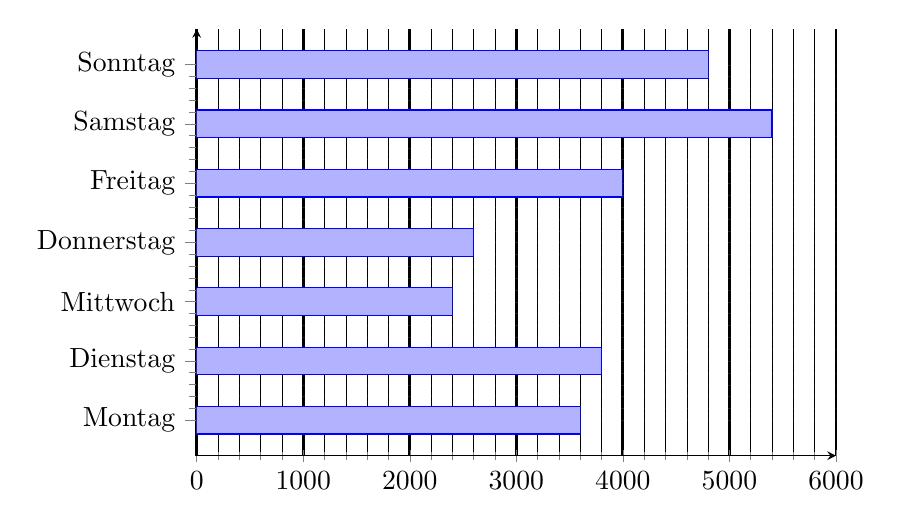
\begin{tikzpicture}
  \begin{axis}[/pgf/number format/1000 sep={},xmajorgrids,xminorgrids, axis lines=left,
  	grid=both,minor tick num=4, major x grid style={line width=1pt,draw=black},
				minor x grid style={line width=.2pt,draw=black}, y grid style={line width=.001pt,draw=white}, xbar,xtick={0,1000,2000,3000, 4000, 5000, 6000},xmin=0,xmax=6000,
    width=0.8\textwidth, height=7cm, enlarge y limits=0.1,
        symbolic y coords={Montag,Dienstag,Mittwoch, Donnerstag, Freitag, Samstag, Sonntag},
    ytick=data,
   nodes near coords align={horizontal},
    ]
    \addplot coordinates {(3600,Montag) (3800,Dienstag) (2400,Mittwoch) (2600,Donnerstag) (4000,Freitag) (5400,Samstag) (4800,Sonntag)};
  \end{axis}
\end{tikzpicture}

\leer

Berechne den durchschnittlichen Tagesumsatz f�r diese Woche.


\antwort{\leer

$\dfrac{4\,800 + 5\,400 + 4\,000 + 2\,400 + 3\,800 + 3\,600}{7}=3\,800$\leer

Der durchschnittliche Tagesumsatz betr�gt \euro\,3.800.}
\end{beispiel}